\chapter{Analysis: Limit calculation}
\label{ch:limit}

In both the \eejj~and \enujj~channels, 
the number of observed data events passing the full selection criteria is consistent with the 
standard model background prediction.
In the absence of a leptoquark signal, an upper limit on the leptoquark production cross section times 
branching fraction is set using the asymptotic CL$_{\text{S}}$ modified frequentist 
approach~\cite{cls-1,cls-2}.

The 95\%~C.L. upper limit on $\sigma \times \beta^2$ (for the \eejj~channel) and 
$\sigma \times 2\beta(1-\beta)$ (for the \enujj~channel) as a function of 
leptoquark mass are shown together with the NLO predictions for the scalar leptoquark pair production cross section 
in Figure~\ref{fig:limits-1D}.
By comparing the observed upper limit with the theoretical cross section values, 
first generation scalar leptoquarks with mass less 
than \ObservedLimitBetaOneeejj~(\ObservedLimitBetaHalfenujj) GeV are excluded
with the assumption that $\beta = 1(0.5)$. This is to be compared with 
a median expected limit of \ExpectedLimitBetaOneeejj~(\ExpectedLimitBetaHalfenujj)~GeV.

 \begin{figure}[htbp]
  \begin{center}
    \begin{tabular}{c}
      \resizebox{10cm}{!}{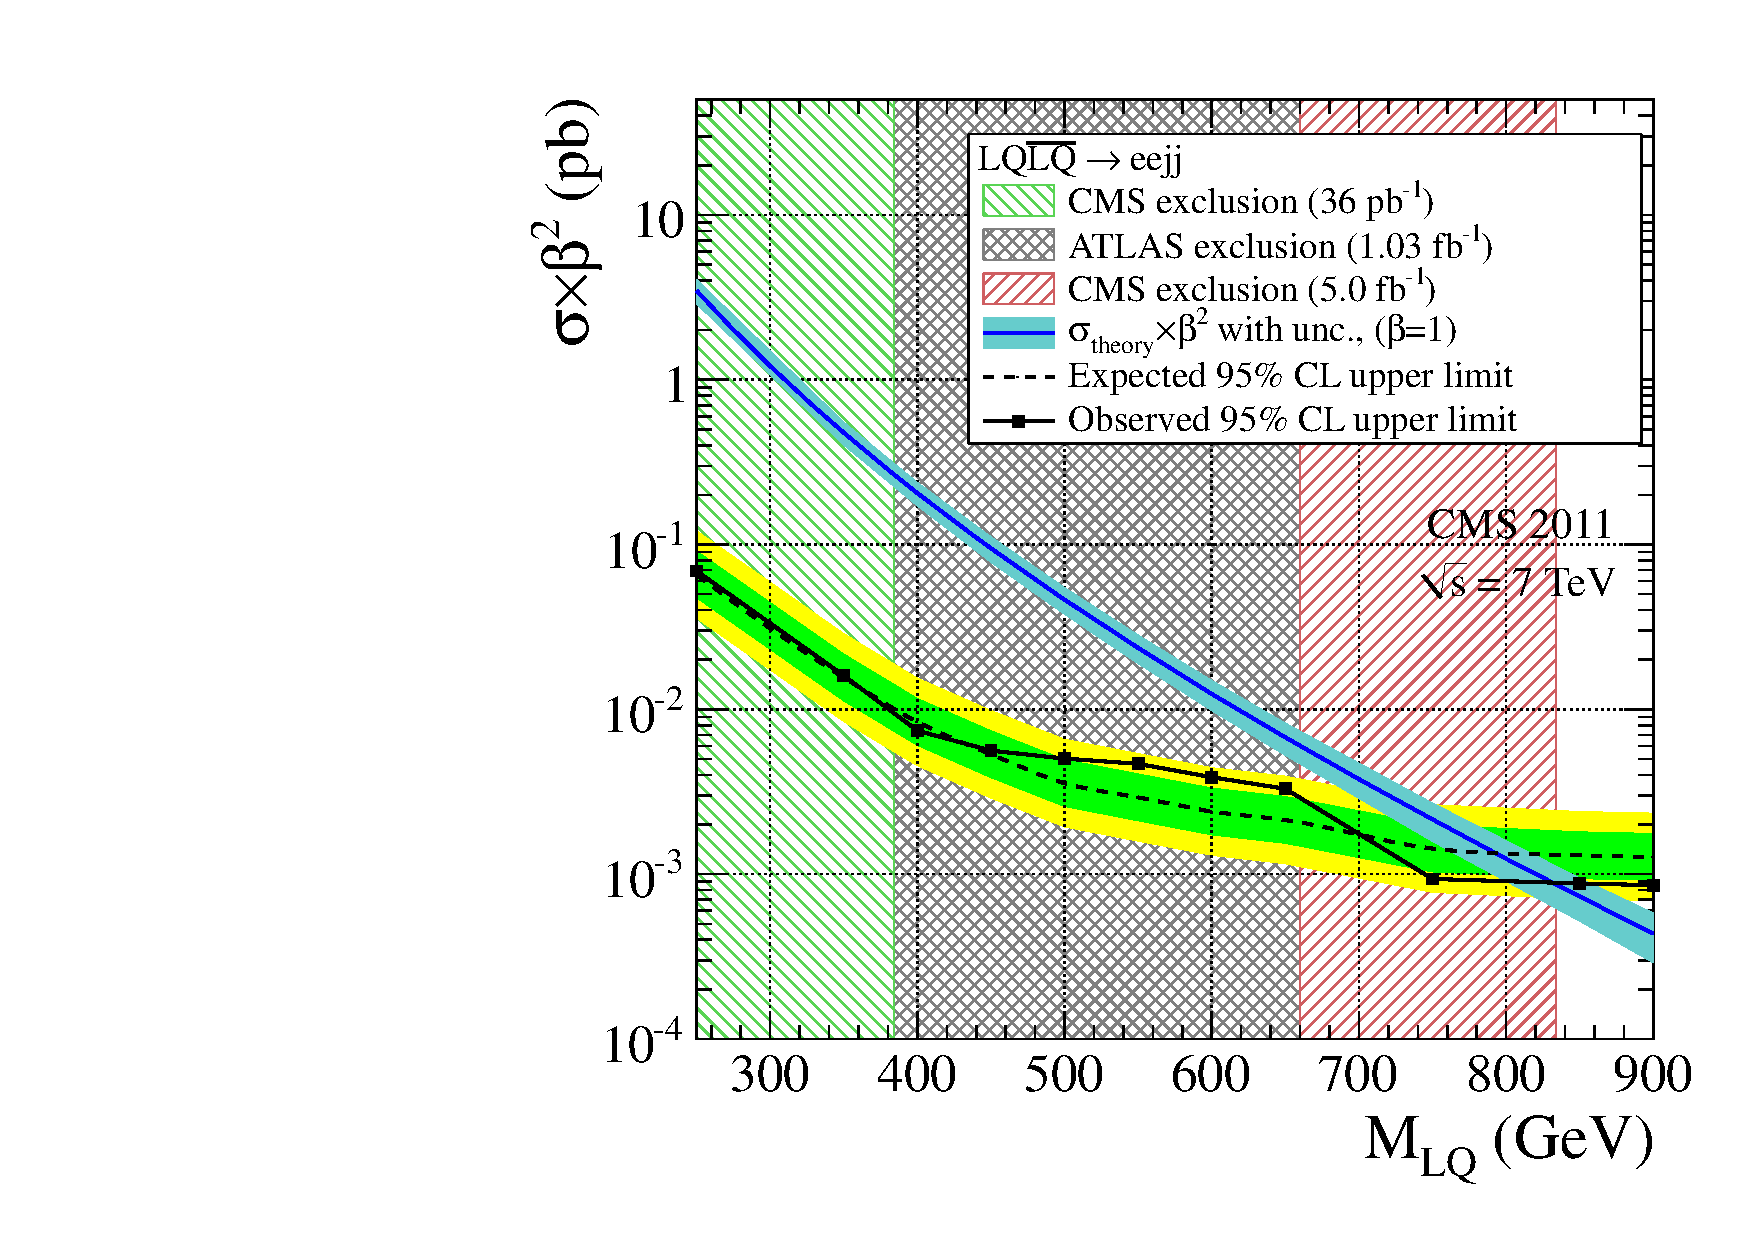
\includegraphics{tex/analysis/results/fig/BR_Sigma_EE.pdf}} \\
      \resizebox{10cm}{!}{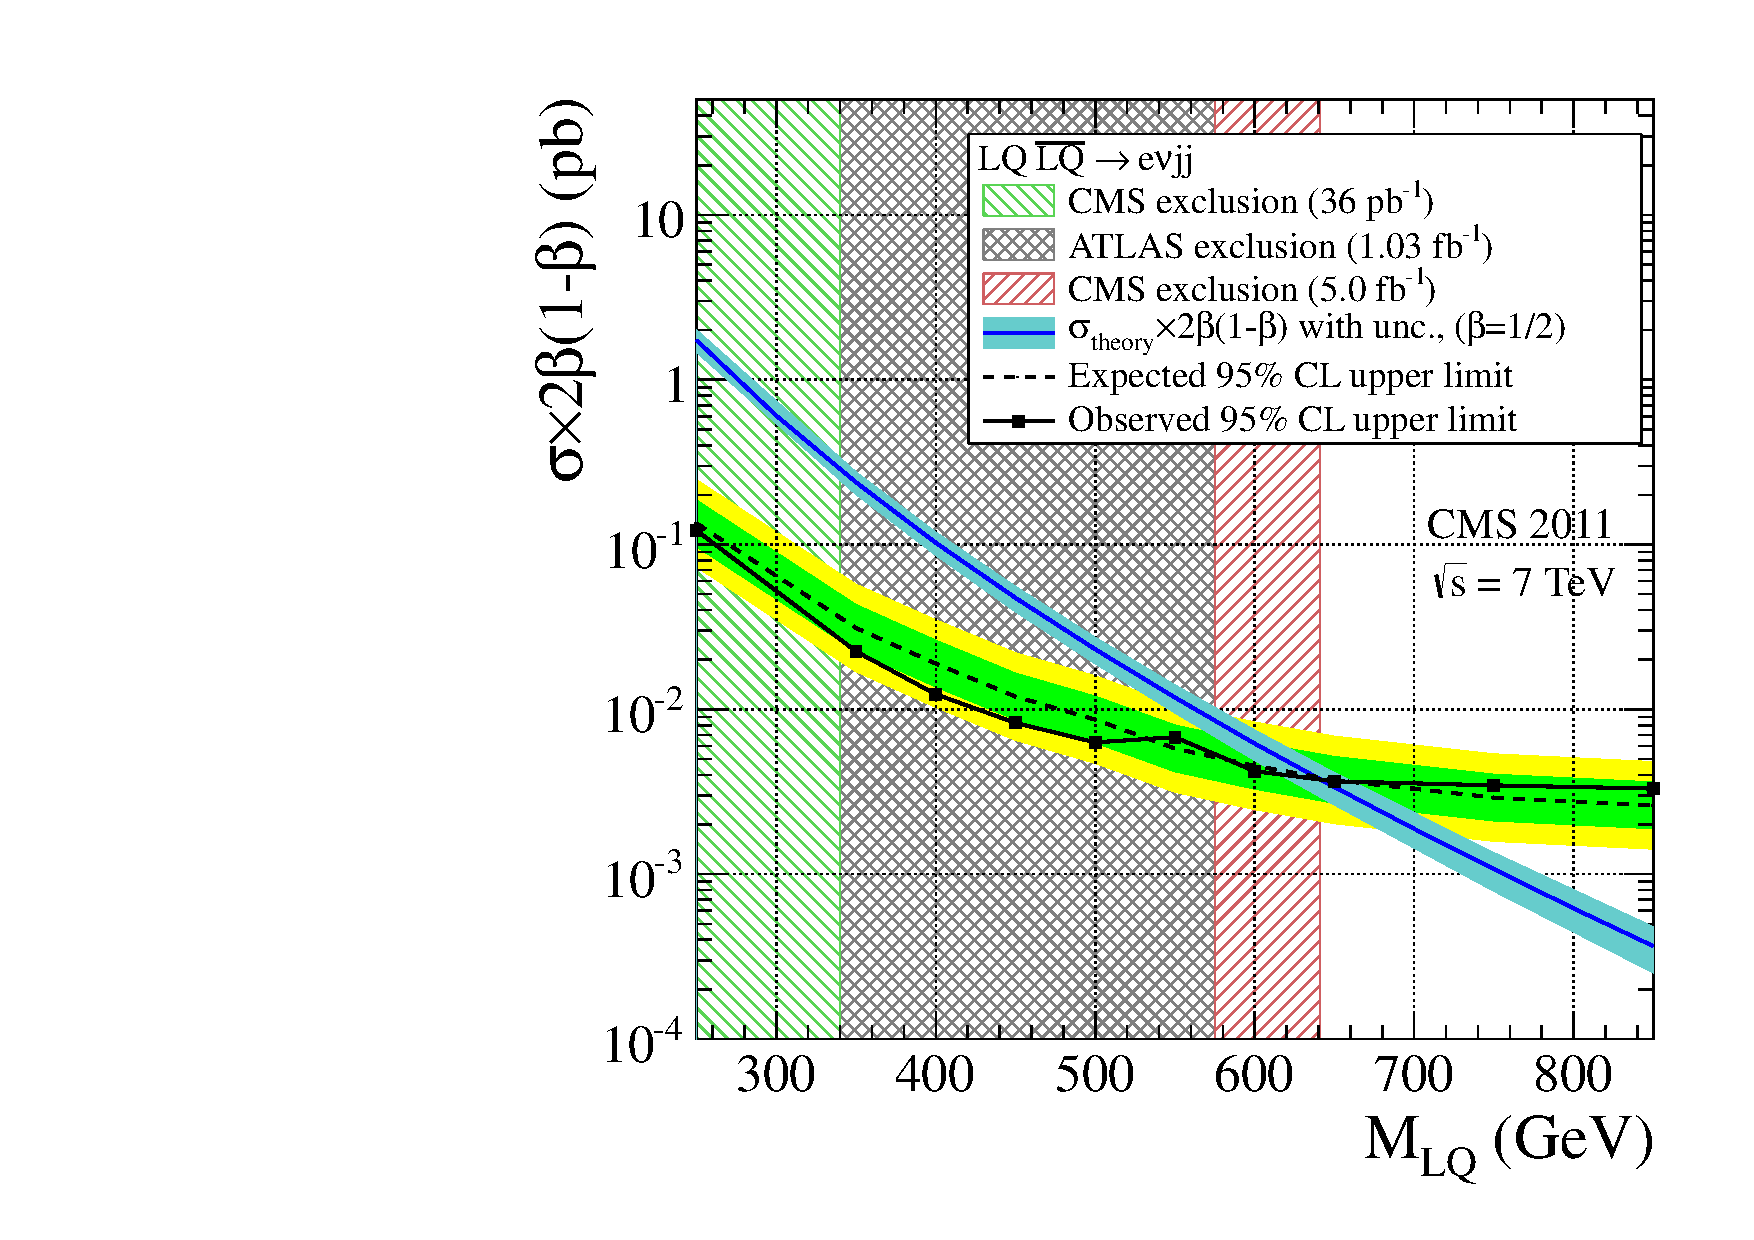
\includegraphics{tex/analysis/results/fig/BR_Sigma_ENu.pdf}} \\
    \end{tabular}
    \caption{The expected and observed upper limit at $95\%$ C.L. on the leptoquark pair production 
    cross section times $\beta^2$ in the top plot ($2\beta(1-\beta)$ in the bottom plot) 
    as a function of the leptoquark mass obtained with the \eejj~(\enujj) analysis. 
    The systematic uncertainties described in the text are included in the calculation.
    The dark blue curve and the light blue band represent, respectively, the theoretical leptoquark pair production cross section 
    and the uncertainties due to the choice of PDF and renormalization/factorization scales~\cite{kramer}.}
    \label{fig:limits-1D}
  \end{center}
\end{figure}   

If a new limit is calculated assuming that the systematical uncertainties
on signal and backgrounds are only coming from the MC statistics, the 
results are very similar to the ones obtained with full systematics.
In particular, no change is observed in the observed lower leptoquark mass limit for 
the \eejj~channel and $\beta = 1$. The lower leptoquark mass limit for the \enujj~channel 
and $\beta = 0.5$ changes from \ObservedLimitBetaHalfenujj~GeV to \ObservedLimitBetaHalfenujjOnlyMCStat~GeV.
This confirms that the limit is dominated by statistical 
fluctuations while systematics play a very small role.

The expected limit on the branching fraction, $\beta$, as a function 
of leptoquark mass may be further improved by combining the \eejj~and \enujj~channels,
as shown in Figure \ref{fig:limit-2D}.  These combinations lead to the exclusion of 
first generation scalar leptoquarks with masses less than \ObservedLimitBetaHalfenujjCombined~GeV
for $\beta = 0.5$, compared with a median expected limit of \ExpectedLimitBetaHalfenujjCombined~GeV.
These limits are currently the most stringent on first generation scalar leptoquarks \cite{pair-lq-CMS}.

\begin{figure}
  \centering
  \resizebox{10cm}{!}{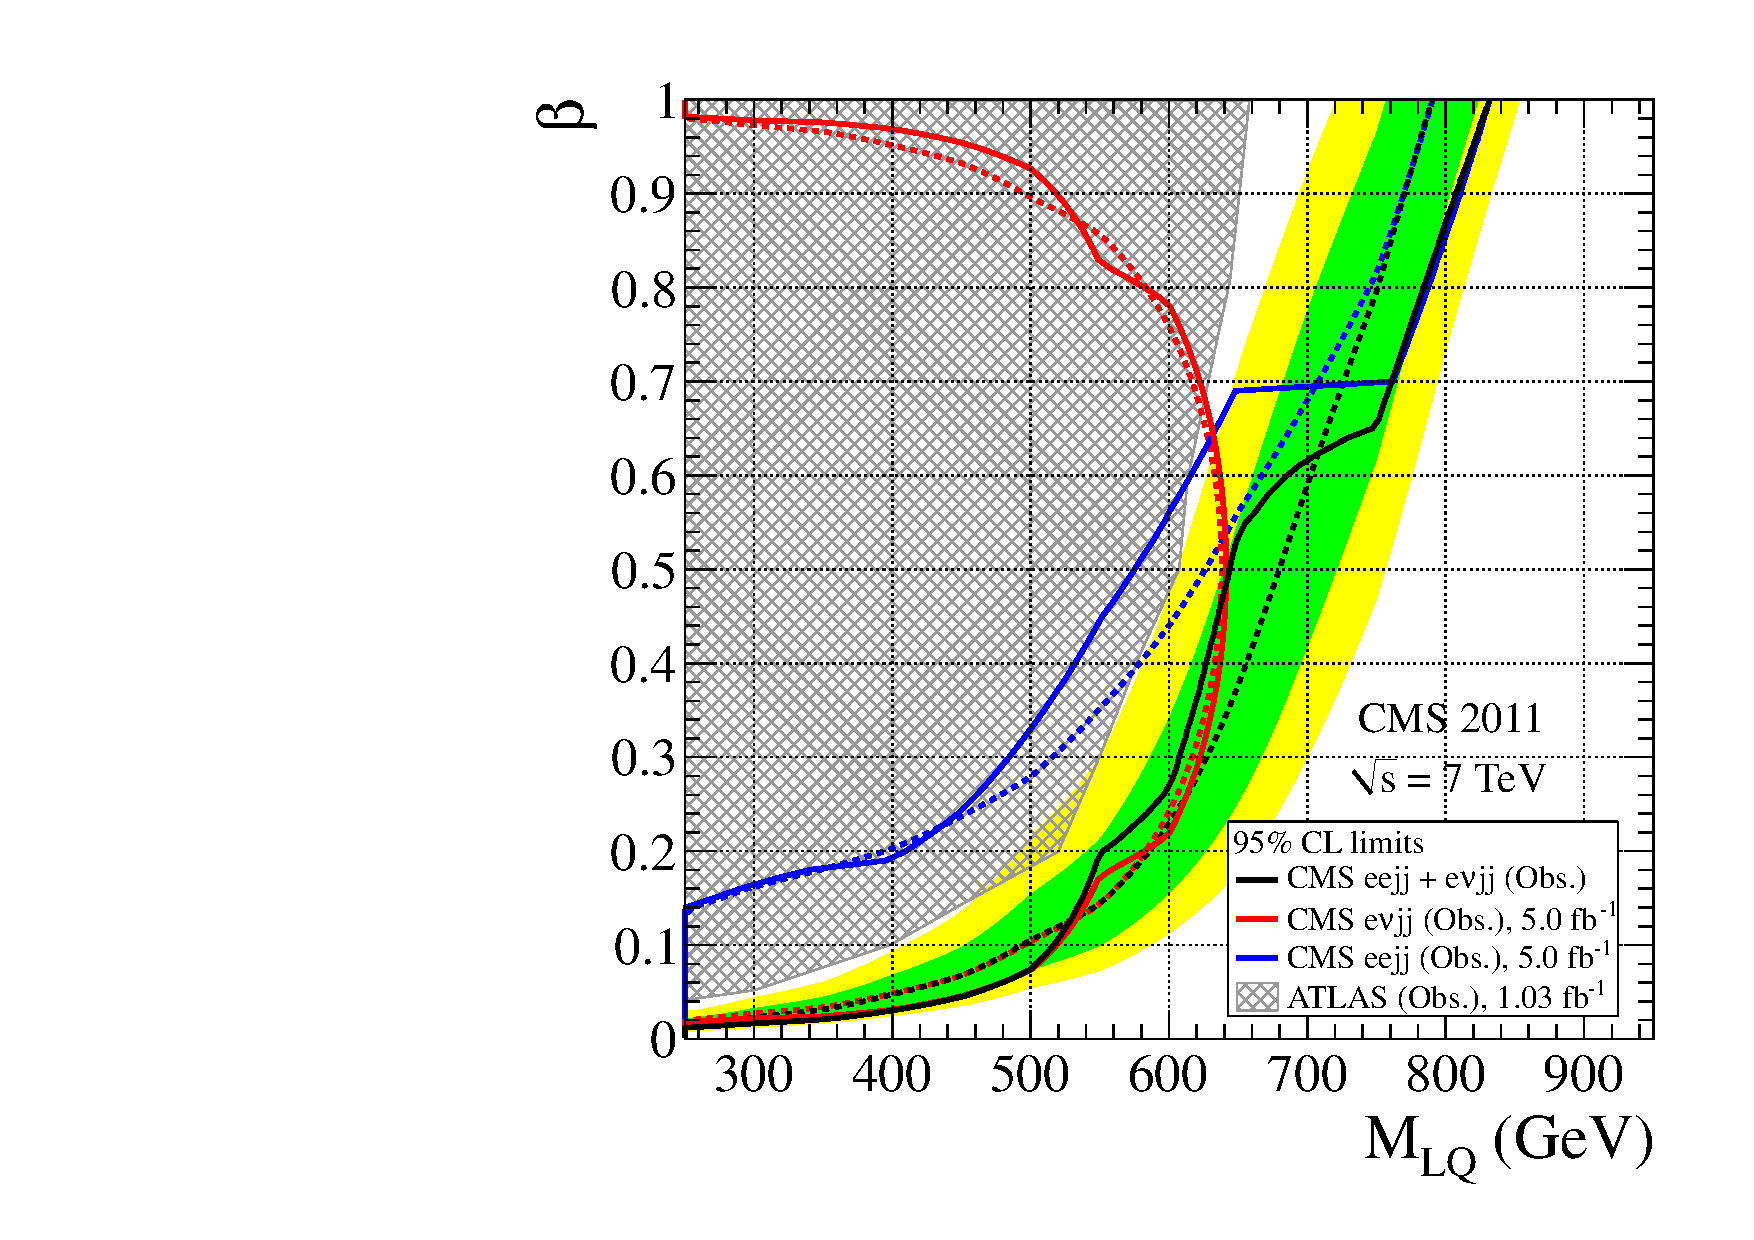
\includegraphics[width=0.95\textwidth]{tex/analysis/results/fig/LQ1Combination.pdf}}
  \caption{The expected and observed exclusion limits at 95\% CL on the first generation leptoquark
    hypothesis in the $\beta$ vs. mass plane using the central value of signal crosss section for the
    individual \eejj~and \enujj~channels and their combination.  The dark green and light yellow expected
    limit uncertainty bands represent the 68\% and 95\% confidence intervals.  Solid lines represent
    the observed limits.  The systematic uncertainties reported in Chapter \ref{ch:analysis-systematics}
    are included in the calculation.  The shaded region is excluded by the current ATLAS limits \cite{pair-lq1-ATLAS}.}
  \label{fig:limit-2D}
\end{figure}
